\chapter{\label{chapter6}Discussion}

In this chapter, we discuss the results of the previous chapter in \ref{chapter6:Convergence time}. We look at the VMAC partitioning in \ref{chapter6:vmac evaluation} and examine the number of required FR flow rules in \ref{chapter6:number of flow rules}.

\section{\label{chapter6:Convergence time}Convergence Performance}

As clearly seen in Figure~\ref{fig:noswift} and Figure~\ref{fig:withswift} iSDX with Swift has a much shorter convergence time. At 500'000 prefixes the convergence time is improved by a factor of 60. The convergence time of the iSDX with Swift increases slightly with a higher number of prefixes. As seen in Figure~\ref{fig:activities} with more prefixes more time is spent until the FR rules are pushed into the IXP fabric. We suppose that this is because the participant controller has to process more BGP updates before it can process the FR message, as the FR messages and BGP udpates get sent over the same channel.

The improvement in the convergence time comes at a cost. That is the overhead Swift adds to the processing of a single BGP update. Since the updates get sent to the Swift-BPA module before getting sent to the participant controller it takes iSDX with Swift longer to process a single BGP update. On average it takes iSDX with Swift about 132\,ns longer to process a single BGP update, that is an increase of a factor 1.13. 

\section{\label{chapter6:vmac evaluation}VMAC Evaluation}

Since both the iSDX and Swift use the destination MAC address to encode information, the amount of bits available to the iSDX and Swift encoding is reduced as the space has to be shared. The current VMAC partitioning is simply the first intuition on how the VMAC can be partitioned. The partitioning can easily be changed by adapting the iSDX's configuration parameters. This partitioning is not yet optimal and can certainly be improved. This was not part of this semester thesis. In this section we evaluate the VMAC partitioning in its current state.

\begin{figure}[h]
\center
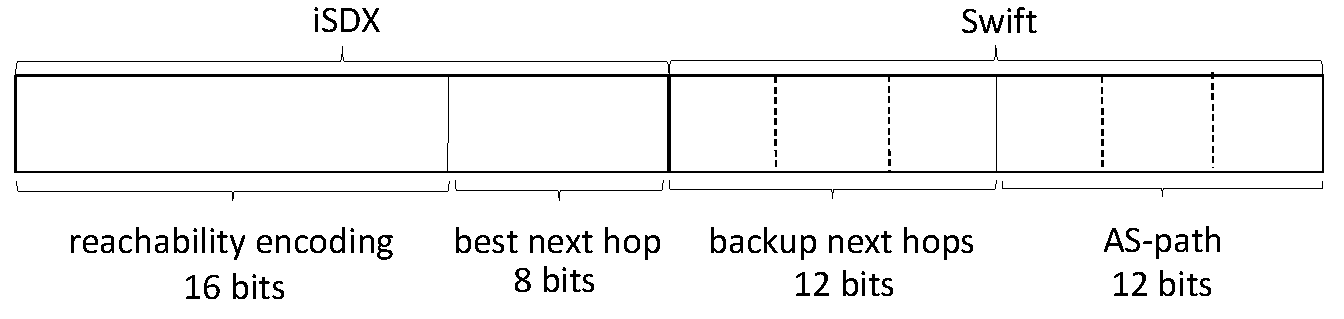
\includegraphics[scale = 0.65]{Figures/eval_vmac2_cropped.pdf}
\caption{Detailed VMAC of the iSDX with Swift}
\label{fig:discussion_VMAC}
\end{figure}

Figure~\ref{fig:discussion_VMAC} show the VMAC partitioning with the number of bits allocated for each part. 
In its current state, 24 bits are allocated to the iSDX: 16 bits for the reachability encoding and 8 bits for the BGP best next hop. 
The amount of bits allocated for the best next hop limits the number of participants the iSDX can have. The number of participants is limited to 2\textsuperscript{8} = 256.

24 bits are allocated to Swift. 12 bits are used to encode backup next hops and 12 bits are used for the AS-path encoding. 
With 12 bits used for the AS-path encoding the encoding has a coverage performance of about 85\%. \cite{swift}
12 bits for 3 backup next hops means that for each next hop 4 bits are used. This means that every participant can have 16 backup next hops at most. This is not a lot and after 16 backup next hops have been assigned some prefixes will end up with no backup next hop. On the other hand, it also limits the number of FR rules.

\section{\label{chapter6:number of flow rules}Fast Reroute Flow Rules}

In this section we will first examine the number of FR flow rules required for a fast reroute in \ref{chapter6:number of flow rules:number_of_Flow_Rules}. We will also examine the priority of the FR flow rules compared to outbound policies in \ref{chapter6:number of flow rules:outbound_FR}

\subsection{\label{chapter6:number of flow rules:number_of_Flow_Rules}Number of Flow Rules}

After a FR message has been received FR rules are pushed into the IXP fabric. The number of FR rules does not depend on the number of withdrawn prefixes. It depends on the number of backup next hops and number of participant controllers. 
In this subsection we examine the number of flow rules required for a fast reroute after a Swift-BPA module detects a failed link. Note that during a burst more than one failed link may be detected. 

For every backup next hop that the participant controller has stored a rule is pushed. This means the maximum number of rules pushed by a participant controller after a fast reroute is 16. 16 is the number of backup next-hops available to every participant (see \ref{chapter6:vmac evaluation}).

FR messages get sent to every participant that is peering with the participant whose Swift-BPA triggered the fast reroute. This means the maximum number of flow rules pushed after a fast reroute is triggered is 256$\cdot$16 = 4096. 256 is the maximum number of participants the iSDX with Swift can have (see \ref{chapter6:vmac evaluation}).

This amount of flow rules is not substantial enough to have a significant impact on the iSDX. With the number of participants limited to 256 and participants having a reasonable number policies, the flow rule limit for current SDN switches should not be reached \cite[Figure 3 (a)]{gupta2016industrial}.

Usually this upper bound of FR rules should not be reached. Upon a fast reroute not all participants will be peering with the participant that triggered the fast reroute. Also the participants may not have reached the maximum number of backup next hops yet.

\subsection{\label{chapter6:number of flow rules:outbound_FR}Outbound Policies and Fast Reroute Rules}

Flow rules have different priorities. Packets get forwarded depending on the flow rule with the highest priority. 
Outbound policies direct packets away from the BGP best path. Swift reroutes packets to backup next hops based on the AS-path of the BGP best path. Hence the question arises, whether in case of a fast reroute all packets that might be affected should be rerouted using Swift or to put it differently which flow rules should have higher priority FR rules or outbound policy rules.

If outbound policies have a higher priority than FR rules, packets that match the policy may be rerouted to a backup next hop or they may be rerouted to a participant whose BGP route traverses the failed AS-link. Packets that do not match the policy will be redirected according to Swift. If FR rules have a higher priority, the participants outbound policies will be ignored in case of a fast reroute.

Due to the limited number of bits available, encoding the AS-path and backup next hops of the participants routes in the reachability encoding is not feasible. In the current iSDX with Swift FR rules have a higher priority than outbound policies. Future studies may allow participants to define which outbound policies they want overridden by Swift and which ones not. But this goes beyond the scope of this project.

